
%% bare_jrnl.tex
%% V1.4b
%% 2015/08/26
%% by Michael Shell
%% see http://www.michaelshell.org/
%% for current contact information.
%%
%% This is a skeleton file demonstrating the use of IEEEtran.cls
%% (requires IEEEtran.cls version 1.8b or later) with an IEEE
%% journal paper.
%%
%% Support sites:
%% http://www.michaelshell.org/tex/ieeetran/
%% http://www.ctan.org/pkg/ieeetran
%% and
%% http://www.ieee.org/

\documentclass[journal]{IEEEtran}


% *** PACKAGES ***
\usepackage{algorithm, algorithmic}
\usepackage{amsmath}
\usepackage{amssymb}
\usepackage{amsthm}
\newtheorem{assumption}{Assumption}
\usepackage{caption}
\usepackage[noadjust]{cite}
\usepackage{color}
\usepackage{enumerate}
\usepackage{mathtools}
\usepackage{url}

% *** GRAPHICS RELATED PACKAGES ***
%
\ifCLASSINFOpdf
\usepackage[pdftex]{graphicx}
  % declare the path(s) where your graphic files are
 \graphicspath{{Figure_1}}
  % and their extensions so you won't have to specify these with
  % every instance of \includegraphics
  \DeclareGraphicsExtensions{.pdf,.jpeg,.png}
\else
  % or other class option (dvipsone, dvipdf, if not using dvips). graphicx
  % will default to the driver specified in the system graphics.cfg if no
  % driver is specified.
  % \usepackage[dvips]{graphicx}
  % declare the path(s) where your graphic files are
  % \graphicspath{{../eps/}}
  % and their extensions so you won't have to specify these with
  % every instance of \includegraphics
  % \DeclareGraphicsExtensions{.eps}
\fi

% correct bad hyphenation here
%\hyphenation{op-tical net-works semi-conduc-tor}

\begin{document}
% Do not put math or special symbols in the title.
\title{Multi-Target Tracking\\ via Mixed Integer Optimization}


% author names and IEEE memberships
\author{Dimitris~Bertsimas,~Zachary~Saunders, and Shimrit~Shtern}

% make the title area
\maketitle

% As a general rule, do not put math, special symbols or citations
% in the abstract or keywords.
\begin{abstract}
The field of multi-target tracking faces two primary challenges: (i) data association and (ii) trajectory estimation. MTT problems are well researched with many algorithms solving these two problems separately, however few algorithms attempt to solve these simultaneously and even fewer utilize optimization. In this paper we introduce a new mixed integer optimization (MIO) model which solves the data association and trajectory estimation problems simultaneously. Furthermore, we propose a greedy heuristic which provides good solutions very quickly and demonstrate its effectiveness as a warm start to the optimization solver. 
\end{abstract}

% Note that keywords are not normally used for peer review papers.
\begin{IEEEkeywords}
optimization; multi-target tracking; data association; trajectory estimation; mixed integer optimization 
\end{IEEEkeywords}

\section{Introduction}

\IEEEPARstart{M}{ulti}-target tracking is the problem of estimation the state of multiple dynamic objects, referred to as \textit{targets} over a fixed window of time. At various points of time within the window, the targets are observed in a \textit{scan}, resulting in set of \textit{detections}. From these detections, the multi-target tracking problem aims to extract information about target dynamics. 

Solutions to this problem are sought across many civilian and military applications including but not limited to ballistic missile and aircraft defense, space applications, the movement of ships and ground troops, autonomous vehicles and robotics, and air traffic control. Each application has unique attributes and assumptions, and various algorithms have been developed for each. As a result, the field of multi-target tracking has expanded to numerous research venues, and there is a wide range of literature on the topic.

The field of multi-target tracking faces two primary challenges: (i) data association and (ii) trajectory estimation.  Given a set of sensor detections the data association problem consists of assigning the detections to a set of targets. Alternatively, this can be viewed as a labeling problem in which each detection needs to be labeled with a target identifier. The association problem is further complicated when sensors fail to report detections (missed detection) or incorrectly report detections (false alarm), resulting in ambiguity in the number of existing targets. The trajectory estimation problem consists of estimating the state space of a target (\textit{i.e.}, position, velocity, acceleration, size, etc.) from the associated detections of the aforementioned assignment problem. Even when all of the associations are known, the estimation problem is challenging due to the presence of measurement noise. As can be seen, the two problems of data association and trajectory estimation are closely related and dependent on one another. 

Some classical algorithms treat the data association and trajectory estimation problems separately using a combination of probabilistic approaches to determine data associations and filters to estimate trajectories. One such algorithm is the global nearest neighbor (GNN). The GNN algorithm is a naive 2-D assignment algorithm, which evaluates one scan of detections at a time, globally assigning the nearest detection at each scan \cite{GNN}. Once the data association has been determined, the detections are often passed through one of numerous filters, most commonly a Kalman filter \cite{Kalman}, which updates the trajectory estimates before the algorithm progresses forward to the next scan. This process repeats sequentially through each scan of data.

Modern algorithms in the field of multi-target tracking are most commonly statistical based, often relying on heavy probabilistic assumptions about the underlying target dynamics or detection process. The two most prevalent statistical algorithms in the field of multi-target tracking are the the Multiple Hypothesis Tracker (MHT) and the Joint Probability Data Association Filter (JPDAF) and their numerous variants and extensions. Both classes of algorithms attempt to solve the data association problem by generating a set of potential hypotheses, or possible detection-to-track assignments. Here a \textit{track} is a set of labelled detections belonging to the same target. Probabilities are assigned to each hypothesis based on the likelihood of the trajectory's existence, and numerous approaches for accomplishing this task have been proposed.

The MHT, first proposed by Reid in \cite{MHT-Seminal}, assigns likelihood values to hypotheses using a Bayesian MAP estimator, which requires assumptions on object dynamics. This algorithm is generally considered to be the modern standard for solving the data association problem. Many variants have been proposed for implementation which leverage techniques such as clustering, gating, hypothesis selection, hypothesis pruning, and merging of state estimates. Many of these methods are summarized by Blackman in \cite{MHT-Overview}. 

While the MHT has seen various forms of success, it faces several key challenges. Namely, the curse of dimensionality and complexity. The number of possible hypotheses grows exponentially with the number of potential tracks and the number of scans. Consequently, it is considered intractable for large scenarios. Moreover, the MHT can be highly tunable and difficult to implement in practice, not to mention computationally expensive. For these reasons it is generally considered to be one of the most complex MTT algorithms. 

A Probability Data Association (PDA) takes a Bayesian approach to solving the data association problem by finding detection-to-target assignment probabilities via a posterior PDF, which again requires heavy assumptions on object dynamics and the detection process. In similar fashion, a Joint PDA (JPDA) assigns probabilities that are computed \textit{jointly} across all targets. The JPDAF is an algorithm which implements the JPDA along with filters and estimation methods as discussed previously. \cite{Bar-Shalom_MTT} 

A limited number of operations research algorithms have been applied to solve the MTT problem, most of which attempt to solve by mapping the measurement set onto a trellis and seek the optimal measurement association sequence. Some examples include the Multi-Target Viterbi\cite{Viterbi-1} and an extension in \cite{Viterbi-2} which formulates \cite{Viterbi-1} as a network flow, reducing the solve time from exponential to polynomial. Others have suggested adaptations which allow this approach to be used similar to MHT methods by outputting a single best set of K tracks, or a list of L best sets of k tracks \cite{Viterbi-3}. 

Compared to the number of statistical based algorithms in the MTT literature, optimization based algorithms are relatively lacking. In fact, most occurrences of optimization in the MTT literature propose the use of optimization to leverage statistical algorithms, in particular the MHT. For example, Integer optimization has been used to improve MHT hypothesis selection by solving an assignment problem which chooses the best hypothesis, but only after costs have been assigned (statistical base) and hypothesis have been pruned \cite{MHT-IP}. Somewhat similarly, linear optimization has also been used to assist in the hypothesis selection process for the MHT \cite{MHT-LP}. Still, other attempts aim to improve the MHT hypothesis selection process via Lagrangian relaxation \cite{Lagrangian}. 

More recently, Andriyenko and Schindler have proposed formulating the MTT problem as a minimization of a continuous energy in \cite{Continuous_energy} and then again as a minimization of discrete-continuous energy in \cite{Discrete-Continuous_energy}. These algorithms aim to more accurately represent the nature of the problem, but sacrifice interpretability for complexity in the process. Rather than formulating the problem to lend it easily to traditional global optimization methods, the authors intend to leverage the use of optimization techniques to find strong local minima of their proposed energy objective, and they achieve strong results in doing so. However, this approach calls for the use of several parameters that must be tuned and few recommendations are provided for how to go about such a tuning process. Additionally, these methods require initialization heuristics to begin the solving process. 

There is no shortage of literature on MTT methodologies. A more complete overview of all MTT methods, including the classes of algorithms and their variants as well as additional methods not discussed in this paper, can be found in \cite{MTT-Taxonomy}. For a more exhaustive overview of estimation techniques, filtering, gating, and more please see \cite{Bar-Shalom_MTT} or \cite{Bar-Shalom_Estimation}.

In this paper we propose the use of mixed integer optimization (MIO) to formulate and solve the multi-target tracking problem. Although MIOs are generally thought to be intractable (NP-Hard), in many practical cases near optimal solutions and even optimal solutions to these problems can be obtained in reasonable time \cite{Computation}. This can be attributed to the fact that MIO solvers have seen significant performance improvements in recent years due to advancements in both methodology and hardware. The development of new heuristic methods, discoveries in cutting plane theory, and improved linear optimization methods have all contributed to improvements in performance \cite{Gurobi-MIP}. Modern solvers such as Gurobi and CPLEX have been shown to perform extremely well on benchmark tests. In the past six years alone, Gurobi has seen performance improvements by a factor of 48.7 \cite{Gurobi-Benchmark}. CPLEX saw improvements by a factor of 29,000 from 1991 to 2007 \cite{CPLEX-Benchmark}. From 1994 to 2014, the growth of supercomputing power as recorded by the TOP500 list has improved by a factor of 567839 \cite{Supercomputer}. Thus, the total combined effective improvement of software and hardware advancements is on the scale of 800 billion times in the past 25 years. 

The literature is also lacking in performance metrics for the evaluation of MTT algorithms. There is no standard method of measuring scenario complexity or algorithm performance as a function of this complexity. In many cases only the sensor's detection noise is taken into account and other factors such as target density is negated. Recent work \cite{MTT-Performance} proposes a mathematically rigorous performance metric for measuring the distance between ground truth and estimated track, but there is not much attention given to the complexity of generated scenarios. In this paper we also suggest measures of complexity and performance which are related to the ones suggested in \cite{MTT-Performance} but we show the value in relating a complexity measure to performance measures, namely that it allows you to evaluate the data association and trajectory estimation problems separately. We evaluate the methods suggested in this paper using these complexity and performance measures on two simulated experiments.

In this work we aim to simultaneously solve the data association and trajectory estimation problems via global optimization using a single interpretable MIO model which can be solved in practical time for the applications considered. We propose a heuristic that gives us feasible solutions to this problem and show how it can be used as warm start to the MIO in order to improve the quality of the solutions obtained as well as the running time. The main contributions of this paper are as follows: (\textit{i}) we introduce a simple interpretable MIO model which solves the data association and trajectory estimation problems simultaneously for a sensor with no detection ambiguity. (\textit{ii}) We extend this basic model for the case of detection ambiguity, i.e., the case where there are both missed detections and false alarms, keeping interpretability while only adding two tunable parameters, as well as provide general guidelines as to how tune this parameters. (\textit{iii}). we present several measures of scenarios complexity algorithms performance, and discuss the connection between these measures, in order to create a performance threshold for our algorithm. 

The paper structure is as follows. We begin with a description of the MTT problem as we wish to model it in Section II. In Section III we develop a simple MIO formulation for a sensor with no detection ambiguity and extend it to a generalized formulation. Following is a discussion on a proposed heuristic in Section IV. Then we propose extensions for both the MIO formulation and the heuristic to a sensor with detection ambiguity in Section V. Metrics for measuring scenario complexity and algorithm performance are proposed in Section VI. Experimental simulations are outlined in Section VII. A summary of significant computational results are discussed in Section VIII. Finally, conclusions and future work are discussed in Section IX.

{\bf General Notations:}
Unless specified otherwise, $\|\cdot\|$ is used to indicate the L1 norm, and $|\cdot|$ refers to element wise absolute value.

\section{Problem Description}
In this paper, we restrict our exploration of the MTT problem to the automatic tracking of multiple, independent point targets using a single sensor. A \textit{target} is the object of interest. A point target's only identifiable attributes are its state space, which we restrict to position and velocity. The state space fully defines the field of \textit{trajectories}, or paths along which targets travel. A \textit{detection} is collected from each target at sequential scans. Detections are subject to noise. We treat two general scenarios: with and without detection ambiguity. 

When there is no detection ambiguity, the sensor produces exactly one detection for each target at each time, and there is no other source of detections. Therefore, the number of detections at each point in time is the same as the number of targets, and the data association problem at each point in time is equivalent to a simple assignment problem. Our basic optimization model, presented in section [add reference] will this with this problem. 

Detection ambiguity refers to the more complex case where the sensor generates both false alarms and missed detections. A \textit{False Alarm} occurs when a detection is collected when no target exists. This could be the result of measurement error or difficulties in signal processing. A \textit{Missed Detection} occurs when a data point is not collected at a given time when a target actually exists. Therefore, the number of detections at each point in time may be either higher or lower than the actual number of targets, and each detection can be classified in either of these categories in addition to assigning targets to trajectories as before. In section [add reference] we will extend the formulation of basic model to a robust formulation dealing with this ambiguity, and refer to it as the robust MIO model.

Throughout the paper we make the following assumptions:
\begin{assumption}\label{ass:general_assumption}
\begin{enumerate}[(i)]
\item{}All targets have constant velocity. \textit{i.e.}, Targets do not maneuver and no outside forces act on them.
\item Each target's dynamics are independent of one another.
\item The number of targets remains constant throughout the window of observation, \textit{i.e.}, there is no birth/death of targets.
\item Each target produces at most one detection per scan.
\item The detection errors are independent of one another.
\end{enumerate}
\end{assumption}

{\bf Notation:}
We observe $P$ targets over a fixed time window over which $T$ scans are collected. Scans occur at a fixed rate, usually of about 1Hz, such that the set of scans is denoted by $\{t_{1}, t_{2},...,T\}. $ The $i^{th}$ detection of the $t^{th}$ scan is indicated by $x_{it}$, such that a scan of data at time \textit{t} is the unordered set of detections $\mathcal{X}_{t} = \{x_{1t}, x_{2,t},...,x_{P,t}\}$. The data for the problem is the ordered set of scans $\boldsymbol{\mathcal{X}}=\{\mathcal{X}_{1},\mathcal{X}_{2},...,\mathcal{X}_{T}\}$. The state space of target trajectories is paramatarized by a true initial position $\alpha^{true}_{j}$ and a true constant velocity $\beta^{true}_{j}$. Therefore, the true position $\bar{x}_{jt}$ of trajectory $j$ at scan $t$ is given by: 

\begin{align}
	\bar{x}_{jt} = \alpha^{true}_{j} + \beta^{true}_{j}t
\end{align}

\section{Basic MIO Model}

In this section, we deal with the case of no detection ambiguity. Therefore, we add the following, more restrictive assumptions, to those presented in Assumption~\ref{ass:general_assumption}
\begin{assumption}\label{ass:basic_assumptions}
\begin{enumerate}[(i)]
\item The sensor generates exactly one detection for each target at each time (no missed detections).
\item The sensor does not generate any additional detections (no false alarms).
\end{enumerate}
\end{assumption}

We begin constructing our MIO model by defining decision variables that represent the desired detection to target associations and target estimated trajectories. Next, using these decision variables, we develop an objective function which mathematically quantifies the value of the model decisions, in this case as a measure of distance of the estimated trajectories from the associated detections. Finally, we restrict these variables using constraints that force the model to find solutions that are feasible for the MTT problem. The model is developed step by step in the coming sections before the full model is presented. 

\subsection{Decision Variables}
The data association and trajectory estimation problems require unique decision variables. Because these two problems lie in different domains, the variables we use to represent these decisions also differ. First, we introduce \textit{continuous} decision variables $\alpha_{j} \in \mathbb{R}^n$ and $\beta_{j} \in \mathbb{R}^n$ to represent the estimated initial position and velocity of each trajectory \textit{j}.  In our interpretation of the MTT problem we allow the trajectory parameters to lie anywhere in the real-continuous domain. For the data estimation problem, we wish to assign detections to trajectories, a naturally discrete problem. Therefore, we introduce binary decision variables $y_{itj}$ to indicate whether detection $x_{it}$ is assigned to trajectory \textit{j} or not:
\begin{align}
y_{itj} =
\begin{cases}
1, & \text{if detection $x_{it}$ is assigned to trajectory \textit{j},} \\
0, & \text{otherwise.}
\end{cases}
\end{align}

\subsection{Objective Function}
Next, we would like to develop a function which accurately scores the quality of a feasible solution. An ideal objective function would jointly provide a single quantifiable measure of goodness for both the data association and trajectory estimation problems. Therefore we want the objective to take into account the assignments of detections in addition to the estimated trajectory determined by those assignments.

In terms of our established decision variables, the estimated position of the linear trajectory \textit{j} at time \textit{t} is given by:

\begin{align}\label{eq:estimate_pos}
	\hat{x}_{jt} =  \alpha_{j} + \beta_{j}t
\end{align}

For the trajectory estimation problem we wish to minimize the distance between $x_{it}$ and $\hat{x}_{jt}$. In other words, for detections $x_{it}$ assigned to trajectory $j$, we wish to minimize $\|x_{it} - \hat{x}_{jt}\|$ for some norm. The two natural norms to consider here are the L1 and L2 norms. The L1 norm has the advantage that it can be reformulated using linear optimization (through the addition of continuous variables and constraints), and it is well known to be more robust to outliers. Additionally, existing algorithms for MIO are more well developed for linear rather than quadratic optimization. However, the L2 norm square form (RSS) has the advantage that it can be quickly computed using a matrix formulation, making it more predisposed to a heuristic. This concept will be discussed further in section IV.

Substituting \eqref{eq:estimate_pos} for $\hat{x}_{jt}$ we arrive at our objective function:
\begin{align}
\underset{\alpha_{j}, \beta_{j}}{\text{minimize: }} & \sum_{(i,j)\in \mathcal{A}} \sum_{t=1}^{T} \|x_{it} - \alpha_{j} - \beta_{j}t\| 
\end{align}
where $\mathcal{A}$ is the set of pairs that indicate the assignment of detection \textit{i} to trajectory \textit{j}.
 
For the data association problem, we wish to only penalize the objective function when detection $x_{it}$ has been assigned to trajectory \textit{j}, which occurs when $y_{itj}=1$. An easy method to enforce this using our established variables would be to construct an interaction term like in \eqref{eq:simple_objective} below. 

\begin{align}\label{eq:simple_objective}
\underset{y_{itj}, \alpha_{j}, \beta_{j}}{\text{minimize: }} & \sum_{i=1}^{P} \sum_{t=1}^{T} |y_{itj}x_{it} - \alpha_{j} - \beta_{j}t\|
\end{align}

We now show that this objective can be converted to a linear program in the case of the L1 norm by introducing continuous variables $\theta_{jt}$ and the following additional constraints. 

\begin{align}
y_{itj}x_{it} - \alpha_{j} - \beta_{j}t \leq \theta_{jt} \qquad \forall i,j,t\\
-(y_{itj}x_{it} - \alpha_{j} - \beta_{j}t) \geq \theta_{jt} \qquad \forall i,j,t
\end{align}

The resulting objective function for the case of the L1 norm would then be:
\begin{align}
\underset{\theta_{jt}}{\text{minimize: }} & \sum_{j=1}^{P} \sum_{t=1}^{T} \theta_{jt}
\end{align}
where $e$ is the vector of ones. 

For the case of the L2 norm, the objective function would be:
\begin{align}
\underset{\theta_{jt}}{\text{minimize: }} & \sum_{j=1}^{P} \sum_{t=1}^{T} {\|\theta_{jt}\|}^{2}_{2}
\end{align}


\subsection{Constraints}
At each time step, each detection $x_{it}$ must be assigned to exactly one target \textit{j}:
\begin{align}
\sum_{j=1}^{P} y_{itj} = 1 \qquad \forall i,t
\end{align}

Similarly, at each time step, each target must be assigned exactly one detection:
\begin{align}
\sum_{i=1}^{P} y_{itj} = 1 \qquad \forall j,t
\end{align}

\subsection{Simple Formulation}
Combining all of these elements together, we arrive at the following MIO model:
\begin{align*}
\underset{\theta_{jt}}{\text{minimize: }} & \sum_{j=1}^{P} \sum_{t=1}^{T} \theta_{jt} \\
\text{subject to: }	& \sum_{j=1}^{P} y_{itj} = 1 \qquad \forall i,t\\
				& \sum_{i=1}^{P} y_{itj} = 1 \qquad \forall j,t\\
				& y_{itj}x_{it} - \alpha_{j} - \beta_{j}t \leq \theta_{jt} \qquad \forall i,j,t\\
				& -(y_{itj}x_{it} - \alpha_{j} - \beta_{j}t) \geq \theta_{jt} \qquad \forall i,j,t\\
			 	& y_{itj} \in \{0,1\} \quad \forall i,t,j\\
				& \alpha_{j} \in \mathbb{R}^n \quad \forall j,\quad \beta_{j} \in \mathbb{R}^n \quad \forall j, \quad z_{jt} \in \mathbb{R}^n \quad \forall j,t\\
\end{align*}

\subsection{Generalized Formulation}
The previous formulation, although simple and easily interpretable, has the disadvantages of being (\textit{i}) dense and (\textit{iI}) ill suited for extension to detection ambiguity. Therefore, next, we present a generalized formulation which can be linearized through the introduction of additional binary decision variables. Alternatively, we can create a new variable $z_{jt}$ which takes on the value $x_{it}$ when $y_{ijt}=1$ and some arbitrary number when $y_{itj}=0$. Using this method we must adjust the objective function below. 

\begin{align}\label{eq:generalized_objective}
\underset{z_{jt}, \alpha_{j}, \beta_{j}}{\text{minimize: }} & \sum_{j=1}^{P} \sum_{t=1}^{T} \|z_{jt} - \alpha_{j} - \beta_{j}t\|
\end{align}

This objective can then be linearized by again introducing $\theta{jt}$ and similar constraints as follows. 
\begin{align}\label{eq:generalized_linear_objective}
\underset{\theta_{jt}}{\text{minimize: }} & \sum_{j=1}^{P} \sum_{t=1}^{T} \theta_{jt}
\end{align}
\begin{align}
z_{jt} - \alpha_{j} - \beta_{j}t \leq \theta_{jt} \qquad \forall i,j,t\\
-(z_{jt} - \alpha_{j} - \beta_{j}t) \geq \theta_{jt} \qquad \forall i,j,t
\end{align}
 
Furthermore, we must ensure that the decision variable $z_{jt}$ will only take on the value of $x_{it}$ in the objective function if $x_{it}$ is assigned to target \textit{j} ($y_{itj} = 1$). We enforce this effect using the following constraint:

\begin{align}
M_{t}(1-y_{itj}) \geq |z_{jt} - x_{it}y_{itj}| \qquad \forall i,t,j\\
\end{align}

where $M_{t} = \underset{j}{\text{max}}|x_{it}|$ for each time step. Furthermore, we can write this equivalently as a linear optimization problem by using the following set of two linear constraints:

\begin{align}
x_{it}y_{itj} + M_{t}(1-y_{itj}) \geq z_{jt} \qquad \forall i,t,j\\
x_{it}y_{itj} - M_{t}(1-y_{itj}) \leq z_{jt} \qquad \forall i,t,j
\end{align}

Combining all of these elements together, we arrive at the following generalized MIO model:
\begin{align*}
\underset{\theta_{jt}}{\text{minimize: }} & \sum_{j=1}^{P} \sum_{t=1}^{T} \theta_{jt} \\
\text{subject to: }	& \sum_{j=1}^{P} y_{itj} = 1 \qquad \forall i,t\\
				& \sum_{i=1}^{P} y_{itj} = 1 \qquad \forall j,t\\
				& x_{it}y_{itj} + M_{t}(1-y_{itj}) \geq z_{jt} \qquad \forall i,t,j\\
				& x_{it}y_{itj} - M_{t}(1-y_{itj}) \leq z_{jt} \qquad \forall i,t,j\\
				& z_{jt} - \alpha_{j} - \beta_{j}t \leq \theta_{jt} \qquad \forall i,j,t\\
				& -(z_{jt} - \alpha_{j} - \beta_{j}t) \geq \theta_{jt} \qquad \forall i,j,t\\
			 	& y_{itj} \in \{0,1\} \quad \forall i,t,j\\
				& \alpha_{j} \in \mathbb{R}^n \quad \forall j,\quad \beta_{j} \in \mathbb{R}^n \quad \forall j, \quad z_{jt} \in \mathbb{R}^n \quad \forall j,t\\
\end{align*}


\section{Heuristic}
Next, we present a detailed description of an algorithm which finds good feasible solutions. These solutions can be used as a warm start to the MIO, providing a performance boost to the MIO. The algorithm hinges on a single heuristic which makes decisions that lead to locally optimal solutions. If the algorithm is repeated with numerous starting points, the best locally optimal solution is kept. 

An important distinction to discuss here is the difference in objective functions. As discussed before the two natural choices are the L1 and L2 norms. For the heuristic, we desire an objective which can be calculated efficiently. Therefore, in this case the L2 norm square (RSS) is the preferred choice because it can be calculated quickly using matrix algebra. \cite{RSS-Matrix} shows how a design matrix M can be using to quickly compute the RSS. 

The algorithm is presented in Algorithm 1. The algorithm initializes by randomizing a solution which satisfies equations 6 and 7. The initial  parameters $\alpha_{j}$ and $\beta_{j}$ are calculated as well as the objective score, $RSS^{0}$. In swap $k$ for scan $t$ choose $i,l\in \{1,\ldots,P\}$ detections and $j,m\in\{1,\ldots,P\}$ targets such that $y^k_{itj}=1$ and $y^k_{ltm}=1$. Switch the detection association so that $y^{k+1}_{ltj}=1$ and $y^{k+1}_{itm}=1$. Compute $\alpha_{j}, \beta_{j}, \alpha_{m}$, $\beta_{m}$, and $RSS^{k}$. If the objective score improves, the swap is kept, otherwise it is rejected. The heuristic then advances to the next scan where the same process is repeated. The algorithm terminates once it makes a single pass through all scans without accepting a single switch. As we will see in the computational results section, this algorithm runs very efficiently, providing high quality global solutions very quickly. Furthermore, this algorithm can be parallelized by running partitions of the $N$ starting points on separate cores, leading to even greater performance advantages. A proposed pseudocode for the heuristic is provided below. 

\begin{algorithm}
 \caption{Randomized local search with heuristic swaps}
 \begin{algorithmic}[1]
 \renewcommand{\algorithmicrequire}{\textbf{Input:}}
 \REQUIRE $\boldsymbol{\mathcal{X}}$, P, T, $\boldsymbol{M}$
 \\ \textit{Initialization} : Assign random initial assignments for $y^{0}_{itj}$
  \STATE Calculate $\alpha_{j}, \beta_{j} \quad \forall j $
  \STATE Calculate $RSS^{0}$
  \STATE swapped $= true$
  \STATE $ k=1 $
  \WHILE{swapped}
  \STATE swapped $= false$
  \FOR{$t$ in $\{t_{1},t_{2},...,T\}$}
  \STATE Randomly choose $j,m\in\{1,\ldots,P\}$
  \STATE Find $i,l$ such that $y^{k-1}_{itm}=1$ and $y^{k-1}_{ltj}=1$
  \STATE Swap such that $y^{k}_{itj}=1$ and $y^{k}_{ltm}=1$
  \STATE Calculate $RSS^{k}, \alpha_{j}, \beta_{j}, \alpha_{m}, \beta_{m}$
  \IF {($RSS^{k} \geq RSS^{k-1}$)}
  \STATE $y^{k} \leftarrow y^{k-1}$
  \ELSE 
  \STATE swapped $\leftarrow true$
  \ENDIF
  \ENDFOR
  \STATE $ k \leftarrow k + 1 $
  \ENDWHILE
 \RETURN $RSS^{k}, y^{k}_{itj}$ 
 \end{algorithmic} 
 \end{algorithm}

\section{Robust MIO Model}
In this section we treat the case of detection ambiguity. The key difference is that now the number of targets is unknown, and this becomes a third problem which we wish to solve in addition to the data association and trajectory estimation problems which remain once the number of targets has been determined. Since in this case both missed detections and false alarms are present the number of targets is unknown and we may no longer have the same number of detections at each time step. Therefore, we must introduce additional notation for this scenario. We let $n_{t}$ represent  the number of detections at time \textit{t}. We can then identify the fewest and largest number of detections in a time step with $N_{0} = \underset{t}{\text{min }} n_{t}$ and $N_{1} = \underset{t}{\text{max }}  n_{t}$, respectively. 

Specifically, in this case we replace Assumption~\ref{ass:basic_assumptions} by the following less restrictive assumptions.
\begin{assumption}\label{ass:robust_assumptions}
\begin{enumerate}[(i)]
\item The sensor does not generate a detection for any target for any time with probability $P_{d}$ which is constant and independent between targets and scans.
\item At each point in time the sensor generates false alarms according to a Poisson distribution with rate $\lambda_{FA}$, which are located uniformally in the space.
\item The number of true targets $P$ satisfies $N_0\leq P \leq N_1$.
\end{enumerate}
\end{assumption}

We first show that this problem can be solved by dividing it into a subset of simpler problems. We present a MIO formulation that assumes a fixed number of targets. This formulation allows us to leverage the power of parallelization to solve the problem by solving each subproblem separately. The results can then be gathered and compared to find the globally optimal solution. For completeness we also present a formulation which solves the original problem without the need for multiple parallelized MIOs.

\subsection{Fixed Number of Targets (P)}
If we first assume that the number of targets is fixed, we can more easily adapt the generalized formulation presented in Section III to handle the addition of false alarms and missed detections. This simple adaptation requires the introduction of two additional variable types and minimal constraint changes. We can then run these formulations for each possible value of fixed number of targets \textit{P} across the range of $N_{0}$ to $N_{1}$ and choose the solution with the best objective overall. Furthermore, this is an advantageous strategy because each independent experiment can be run in parallel. 

\subsubsection{Decision Variables}

We first introduce new binary decision variables $F_{it}$ to indicate whether or not a detection $x_{it}$ is a false alarm. 

\[F_{it} = 
\begin{cases}
1, & \text{if detection \textit{i} at time \textit{t} is a False Alarm,}\\
0, & \text{otherwise.}
\end{cases}\]

Similarly, we introduce binary decision variables $M_{jt}$ to indicate whether or not an \textit{existing} trajectory \textit{j} has a missed detection at time \textit{t}.

\[M_{jt} =
\begin{cases}
1, & \text{if detection for trajectory \textit{j}}\\
   &\text{at time \textit{t} is a Missed Detection,}\\
0, & \text{otherwise.}
\end{cases}\]

\subsubsection{Constraints}

All detections must either be assigned to a trajectory \textit{j} or a false alarm. 
\begin{align}\label{eqn: FA Simple}
\sum_{j=1}^{P} y_{itj} + F_{it} = 1 \qquad \forall i,t
\end{align}

All trajectories \textit{j} must either be assigned a detection or a missed detection. 
\begin{align}
\sum_{i=1}^{n_{t}} y_{itj} + M_{jt} = 1 \qquad \forall j,t
\end{align}

The sum of all false alarms is TF, and similarly the sum of all missed detections is TM. 
\begin{align}
\sum_{i=1}^{n_{t}} \sum_{t=1}^{T} F_{it} = TF
\end{align}
\begin{align}\label{eqn: MD Total}
\sum_{j=1}^{P} \sum_{t=1}^{T} M_{jt} = TM 
\end{align}

\subsubsection{Objective Function}
We can easily extend \eqref{eq:generalized_objective} to account for false alarms and missed detections by introducing penaties $\psi_{0}$ ($\phi_{0}$, respectively) for each missed detection (false alarm, respectively). Such an objective form would take the form of:
\begin{align}
\underset{z_{jt}, \alpha_{j}, \beta_{j},TF,TM}{\text{minimize: }} & \sum_{j=1}^{P} \sum_{t=1}^{T} \theta_{jt} + \psi_{o} TF + \phi_{0} TM
\end{align}
which can be linearized in the same manner as \eqref{eq:generalized_linear_objective}.

\subsubsection{Formulation 2}

\begin{align*}
\underset{\psi_{jt}}{\text{minimize: }} & \sum_{j=1}^{P} \sum_{t=1}^{T} \psi_{jt} + \theta_{o} TF + \phi_{0} TM\\
\text{subject to: }	& \sum_{j=1}^{P} y_{itj} + F_{it} = 1 \qquad \forall i,t\\
				& \sum_{i=1}^{n_{t}} y_{itj} + M_{jt} = 1 \qquad \forall j,t\\
				& \sum_{i=1}^{n_{t}} \sum_{t=1}^{T} F_{it} = TF\\
				& \sum_{j=1}^{P} \sum_{t=1}^{T} M_{jt} = TM\\
				& x_{it}y_{itj} + M_{t}(1-y_{itj}) \geq z_{jt} \qquad \forall i,t,j\\
				& x_{it}y_{itj} - M_{t}(1-y_{itj}) \leq z_{jt} \qquad \forall i,t,j\\
				& z_{jt} - \alpha_{j} - \beta_{j}t \leq \psi_{jt} \qquad \forall j,t\\
				& -(z_{jt} - \alpha_{j} - \beta_{j}t) \leq \psi_{jt} \qquad \forall j,t\\
				& y_{itj} \in \{0,1\} \quad \forall i,t,j\\
				& \alpha_{j} \in \mathbb{R}^n,\quad \beta_{j} \in \mathbb{R}^n \quad \forall j\\
				& z_{jt} \in \mathbb{R}^n, \quad \forall j,t\\
\end{align*}

\subsection{Number of Targets as a Decision Variable}
In the previous section, we assumed we knew the number of targets. In this section, the number of targets is determined via optimization. 

\subsubsection{Decision Variables}
Toward this goal, we introduce a new binary decision variable $w_{j}$ to indicate whether or not trajectory \textit{j} corresponds to an existing target.

\[w_{j} = 
\begin{cases}
1, & \text{if trajectory \textit{j} exists,}\\
0, & \text{otherwise.}
\end{cases}\]


\subsubsection{Constraints}
Most constraints remain similar to their original counterparts, except now we must account for the possibility that some trajectories may not exist. Therefore, where before we summed over \textit{P}, we will now be summing over $N_{1}$. This affects two constraints.

All detections must either be assigned to a trajectory \textit{j} or a false alarm. This can be implemented similarly to \eqref{eqn: FA Simple}, except now we sum over $N_{1}$ because the number of targets is unknown but limited by $N_{1}$.
\begin{align}
\sum_{j=1}^{N_{1}} y_{itj} + F_{it} = 1 \qquad \forall i,t
\end{align}

Similarly, \eqref{eqn: MD Total} must be adjusted to sum over the maximal number of targets allowed $N_{1}$ . 
\begin{align}
\sum_{j=1}^{N_{1}} \sum_{t=1}^{T} M_{jt} = TM
\end{align}


All \textit{existing} trajectories must either be assigned a detection or a missed detection. 
\begin{align}\label{eqn: Existing Targets}
\sum_{i=1}^{n_{t}} y_{itj} + M_{jt} = w_{j} \qquad \forall j,t
\end{align}

We restrict $\alpha_{j}$ and $\beta_{j}$ to be zero if trajectory \textit{j} does not exist. This ensures only existing trajectories are penalized in the objective function. 
\begin{align}
|\alpha_{j}|+|\beta_{j}| \leq M_{0}w_{j}\qquad \forall j\
\end{align}

Since $N_{0} \leq P \leq N_{1}$, we can set $w_j=1$ for all $j=1,\ldots,N_0$, which leaves us with only $N_1-N_0$ additional binary variables. We simply need the additional constraint
\begin{align}
w_{N_0+1}\geq ...\geq w_{N_1}
\end{align}
which guarantees a unique $w$ solution.
Furthermore, we can replace \eqref{eqn: Existing Targets} with the following two constraints:
\begin{align}
	\sum_{i=1}^{n_{t}} y_{itj} + M_{jt} = 1 \qquad \forall j=1,...,N_{0},t\\
	\sum_{i=1}^{n_{t}} y_{itj} + M_{jt} = w{j} \qquad \forall j=N_{0},...,N_{1},t
\end{align}

\subsubsection{Formulation 3}

Incorporating these additional variables and constraints, we arrive at the following complete alternative formulation.

\begin{align*}
\underset{y_{itj}, \alpha_{j}, \beta_{j},F_{it},M_{jt}}{\text{minimize: }} & \sum_{j=1}^{N_{1}} \sum_{t=1}^{T} |z_{jt} - \alpha_{j} - \beta_{j}t| + \theta_{o} TF + \phi_{0} TM\\
\text{subject to: }	& \sum_{j=1}^{N_{1}} y_{itj} + F_{it} = 1 \qquad \forall i,t\\
				& \sum_{i=1}^{n_{t}} y_{itj} + M_{jt} = 1 \qquad \forall j=1,...,N_{0},t\\
				& \sum_{i=1}^{n_{t}} y_{itj} + M_{jt} = w{j} \qquad \forall j=N_{0},...,N_{1},t\\
				& \sum_{i=1}^{n_{t}} \sum_{t=1}^{T} F_{it} = TF\\
				& \sum_{j=1}^{N_{1}} \sum_{t=1}^{T} M_{jt} = TM\\
				& w_{N_0+1}\geq ...\geq w_{N_1}\\
				& |\alpha_{j}|+|\beta_{j}| \leq M_{0}w_{j}\qquad \forall j\\
				& x_{it}y_{itj} + M_{1}(1-y_{itj}) \geq z_{jt} \qquad \forall i,t,j\\
				& x_{it}y_{itj} - M_{1}(1-y_{itj}) \leq z_{jt} \qquad \forall i,t,j\\
			 	& y_{itj} \in \{0,1\} \quad \forall i,t,j\\
				& \alpha_{j} \in \mathbb{R}^n,\quad \beta_{j} \in \mathbb{R}^n,\quad w_{j} \in \mathbb{R}^n \quad \forall j\\
				& z_{jt} \in \mathbb{R}^n, \quad \forall j,t\\
\end{align*}

\subsection{Adaptation of Heuristic 1}
The heuristic for the scenario with ambiguity follows similarly from the heuristic developed under the scenario without ambiguity. The main difference is that now the options for making switches must include false alarms and missed detections. Therefore, the framework of the algorithm is the same as for Algorithm 1, but now the heuristic randomly chooses from the following options: 
\begin{enumerate}
  \item Switch detection assignments between two existing targets.
  \item Switch the detection assignment of an existing target with a false alarm.
  \item Switch the detection assignment of an existing target with a missed detection for a different existing target.
  \item Move the detection assignment of an existing target to a false alarm and replace it with a missed detection.
  \item Move a false alarm into the location of a missed detection for an existing target.
\end{enumerate}

Similar to Heuristic 1, this algorithm will accept the switch/move if the objective score improves, and reject the switch/move otherwise. The algorithm terminates under the same conditions as Heuristic 1. We expect this algorithm to run slightly slower due to the increase in potential combinations of solutions. 

\section{Scenario Complexity \& Performance Metrics}
There does not exist a unified approach for measuring scenario complexity as stated by \cite{MTT-Taxonomy} nor does there exist an explanation of difficulty as it pertains to each of the MTT problems of data association and trajectory estimation. Here we suggest several metrics which can be used to quantitatively compare the complexity of numerous generated scenarios. Although the two challenges of data association and trajectory estimation are interrelated and we have shown that the two problems can be jointly solved, we argue that it is important to identify measures which score the difficulty of scenarios and performance of results separately. We begin by developing coefficients $\rho$ which is an indicator of the level of complexity and difficulty of a given scenario. The first two metrics aim to capture the difficulty of the estimation problem, however they measure different difficulties. For ease of notation, let 

\begin{align}
D_{ijt} = \| \alpha^{true}_{i} + \beta^{true}_{i}t - \alpha^{true}_{j} + \beta^{true}_{j}t \|
\end{align}

The first proposed measure of $\rho$ aims to capture the average distance between all pairwise trajectories. 

\begin{align}
\rho_{1} = \frac{\sum\limits_{t=1}^{T}\sum\limits_{i<j}D_{ijt}}{\binom{P}{2} T \sigma}
\end{align}

The second measure of $\rho$ aims to capture the average minimal distance between each trajectory and its closest trajectory. 

\begin{align}
\rho_{2} = \frac{\sum\limits_{i=1}^{P} \underset{j} {\text{min}} \sum\limits_{t=1}^{T}D_{ijt}}{P T \sigma}
\end{align}

These metrics have several desirable attributes. For example, the error is equivalent to the noise when $\rho = 1$.  Lower values of $\rho$ correspond to increasingly difficult scenarios, while higher values of $\rho$ correspond to easier scenarios. For a set of fixed trajectories, raising $\sigma$ increases the difficulty, while lowering $\sigma$ decreases the difficulty. 

The last measure of $\rho$ aims to capture the difficulty of the data association problem. Let
\[c_{ijt} = 
\begin{cases}
1 & \text{if $D_{ijt} > 2\sigma$}\\
0 & \text{otherwise}
\end{cases}\]

The metric offers insight into the density of the scenario by measuring the percentage of close proximity detections. 
\begin{align}
\rho_{3} =  \frac{\sum\limits_{t=1}^{T}\sum\limits_{i<j}c_{ijt}}{\binom{P}{2} T}
\end{align}

Similarly, higher values of $\rho_{3}$ indicate easier scenarios because fewer detections are within close proximity, presumably leading to a decreased difficulty in the data association problem. 

Similarly, we propose the use of different metrics to measure the performance of the data association and trajectory estimation problems separately. For the data association problem, which is naturally discrete, we propose the use of \% accuracy \textit{i.e} the ratio of the number of correct detection assignments to the total number of detections detections.
\begin{align}
Accuracy =  \frac{\text{\# correct assignments}}{\text{Total \# of detections}}
\end{align}

Naturally the trajectory estimation problem calls for a performance metric which compares the distance of the ground truth to the estimation trajectory. Therefore, we propose the following metric. 
\begin{align}
	\delta = \frac{\sum\limits_{t=1}^{T}\sum\limits_{j=1}^{P}\| \bar{x}_{jt} - \hat{x}_{jt} \|}{PT}
\end{align}
We match the true trajectories to the estimated trajectories using a one to one assignment problem which can be formulated as a linear program with the absolute distance between true and estimated as label costs.

The classification of simulated scenarios by difficulty and complexity is no easy task, and to the best of the authors' knowledge there is no accepted standard among the MTT community. We have proposed various metrics which allow for the intuitive and quantitative representation of these scenarios. Furthermore, the suggested performance metrics allow us to independently evaluate the performance of MTT algorithms, as it pertains to the data association and trajectory estimation problems. 

\section{Experimental Simulations}
There does not exist among the literature a clearly defined comprehensive set of simulation scenarios as pointed out by \cite{MTT-Taxonomy}.  However, this work also noted that two types of scenarios of particular importance include crossing trajectories and parallel trajectories. In agreement, we choose to develop scenarios of both types. We evaluated our methods on two separate experiments, one with detection ambiguity and one without.

\subsection{Experiment 1}
In order to evaluate scalability we test our methods across a range of scenarios with varying numbers of targets and scans. In particular we consider: $ P \in \{4, 6, 8, 10\}$ and $T \in \{4, 6, 8, 10\}$. Scans are collected at a rate of 1 Hz. The cartesian product of $P$ and $T$ creates 16 unique scenario sizes. We generate 10 unique crossing scenarios and 10 unique parallel scenarios of each size. For each scenario, we randomly generate 10 realizations of data by perturbing the each true position measurement by an error $\epsilon \thicksim \mathcal{N}(0,\sigma)$, where $\sigma$ represents the noise parameter. We generate scenarios with a range of noise parameters $\sigma \in [0.1, 0.5, 1.5, 2.5]$. The problem data is then generated by adding the detection error to the true position.
\begin{align}
	x_{it} = \alpha^{true}_{i} + \beta^{true}_{i}t+\epsilon
\end{align}

Scans $\mathcal{X}_{t}$ are simulated by randomizing the order of $x_{it}$ for each \textit{t}. Each unique $\boldsymbol{\mathcal{X}}$ generated is referred to as a \textit{simulation}. Next, we begin testing our methods feeding the data into our algorithms, starting with the heuristic. For each simulation, we run the heuristic with a range of starting points $N \in \{100\ \ 1,000\ \ 10,000\}$.
Finally, we feed each heuristic solution as a warm start into the MIO and run the optimization solver. The optimization process is set to terminate after 3T seconds, with solutions collected at intervals of $\{1,T,2T,3T\}$ seconds.

\subsection{Experiment 2}
The second experiment serves as an extension of the first in order to test the performance of our algorithms under detection ambiguity. We use the same base data generated from Experiment 1, but now we simulate missed detections and false alarms. 

\subsection{Implementation}
Both experiments were implemented in the development software \textit{julia} 0.4.3 \cite{julia} using the optimization package \textit{JuMP} \cite{JuMP}. The implemented MIO utilized the optimization solver Gurobi 6.5.0\cite{gurobi}. Gurobi was limited to the use of a single core for the optimization processes. Each simulation was run on a single node of the unclassified TX-Green supercomputer located at Lincoln Laboratories \cite{LLGrid}. [Insert computer specs (RAM, CPU, etc.) if available.]

\section{Computational Results}
We begin by outlining the performance of the basic MIO model in both the data association and trajectory estimation spheres. Following is a discussion of the robust MIO model evaluated under both spheres. 


\subsection{Basic Heuristic \& MIO Results}
The performance of the basic heuristic and MIO in the sphere of the data association problem is summarized in Figure 1 below. 
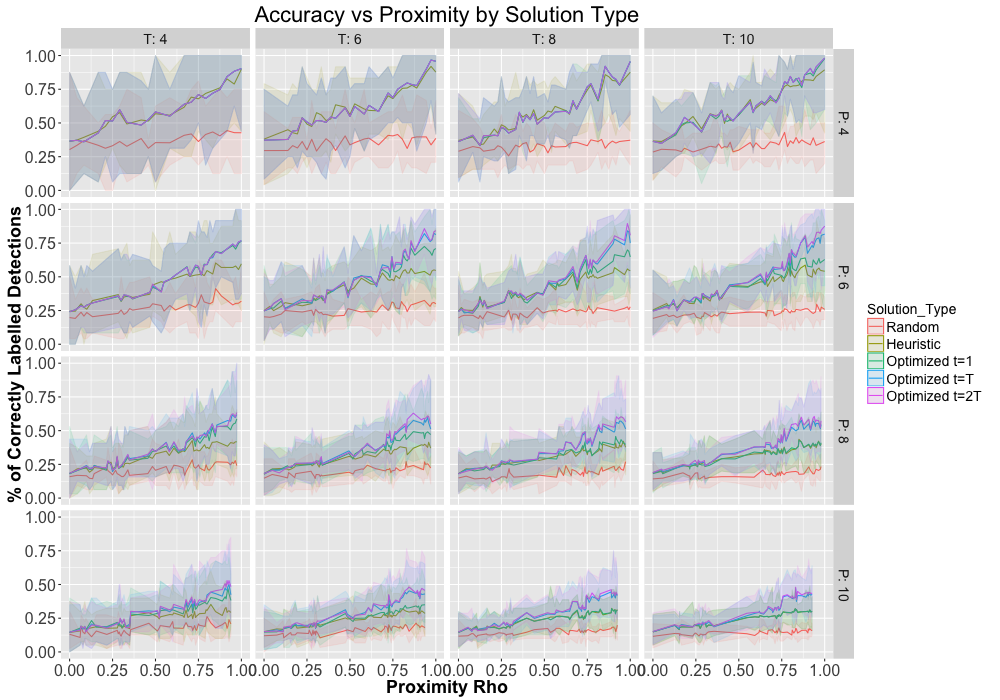
\includegraphics[width=9cm, height=7cm]{Figure_1}
Both are compared to a baseline randomized solution. Figure 1 shows that Heuristic 1 provides improved solutions to the data association problem.  For smaller scenarios of $P$ and $T$, the heuristic achieves optimal and near optimal solutions. We also see that the easier the scenario, the more improvement the MIO has over the heuristic, while in more difficult scenarios the effect is diminished. Furthermore, it can be seen that in nearly all scenarios, the MIO model achieves its best solutions, which could be optimal, after $T$ or fewer seconds, suggesting the usefulness of the MIO as an online algorithm in a sliding window.

Next, we evaluate the performance of the basic heuristic and MIO through the lens of the trajectory estimation problem. Figure 2 summarizes this performance.  

\subsection{Robust Heuristic \& MIO Results}


\section{Conclusion and Future Work}
We presented a multi-target tracking approach which jointly solves the problems of data association and trajectory estimation. We accomplish this without the need of a trajectory bank nor the a prior computation of trajectory hypothesis. We demonstrated that the proposed method outperforms for linear trajectories....

\section*{Acknowledgment}
The authors would like to thank Sung Son, Ph.D and Steve Relyea at Lincoln Laboratories for their efforts in problem clarification as well as for providing feedback and other expert knowledge on the problem details. Additionally, we would like to thank Lincoln Laboratories for and the LLGrid team for its assistance in running our experiments. 


% trigger a \newpage just before the given reference
% number - used to balance the columns on the last page
% adjust value as needed - may need to be readjusted if
% the document is modified later
%\IEEEtriggeratref{8}
% The "triggered" command can be changed if desired:
%\IEEEtriggercmd{\enlargethispage{-5in}}

% references section


% The IEEEtran BibTeX style support page is at:
% http://www.michaelshell.org/tex/ieeetran/bibtex/
%\nocite{*}
\bibliographystyle{IEEEtran}
% argument is your BibTeX string definitions and bibliography database(s)
\bibliography{Bibliography}
%

%\printbibliography

\end{document}